\documentclass{cubeamer}

\title{Performance-Portable Implicit Scale-Resolving Compressible Flow Using libCEED}
\subtitle{SIAM CSE 2023}
\author[James Wright]{James Wright}
\date{February 27, 2023 } % or whatever the date you are presenting in is
\institute[University of Colorado Boulder]{Ann and H.J. Smead Department of Aerospace Engineering Sciences}

\usefonttheme{professionalfonts} % required for mathspec
\usepackage{mathspec}
\setmathsfont{Latin Modern Math}

\usepackage{todonotes}
\presetkeys{todonotes}{inline}{}

\usepackage{minted}

\newminted{c}{fontsize=\tiny,
            linenos,
            numbersep=2pt,
            gobble=0,
            frame=lines,
            bgcolor=bg,
            framesep=3mm}

\renewcommand{\vec}[1]{\bm{#1}}
\newcommand{\defeq}{\vcentcolon=}
\newcommand{\eqdef}{=\vcentcolon}
\DeclarePairedDelimiter{\angbr}{\langle}{\rangle}
\DeclareMathOperator{\Span}{span}
\newcommand{\avg}[1]{\angbr{#1}}

\newcommand<>{\uncoverubrace}[2]{%
  \onslide#3 \underbrace{ \onslide<1->%
  #1%
  \onslide#3 }_{#2} \onslide<1->%
}
\newcommand<>{\uncoverobrace}[2]{%
  \onslide#3 \overbrace{ \onslide<1->%
  #1%
  \onslide#3 }^{#2} \onslide<1->%
}

\usepackage{xcolor}
\newcommand{\Part}{\textcolor[HTML]{ad0000}{\mathcal{P}}}
\newcommand{\PartT}{\textcolor[HTML]{ad0000}{\mathcal{P}^T}}
\newcommand{\Elem}{\mathcal{E}}
\newcommand{\ElemT}{\mathcal{E}^T}
\newcommand{\Bas}{\textcolor[HTML]{0f75ff}{B}}
\newcommand{\BasT}{\textcolor[HTML]{0f75ff}{B^T}}
\newcommand{\DQfunc}{\textcolor[HTML]{009900}{D}}
\newcommand{\nelm}{{n_{\mathrm{elm}}}}
\newcommand{\ndof}{{n_{\mathrm{dof}}}}
\newcommand{\nquad}{{n_{\mathrm{quad}}}}

\begin{document}

\maketitle

\cutoc

\section{What is libCEED?}

\begin{frame}{What is libCEED?}

    \begin{itemize}
        \item<+-> C library for element-based discretizations
            \begin{itemize}
                \item<+-> Bindings for Fortran, Rust, Python, and Julia available
            \end{itemize}
        \item<+-> Designed for matrix-free operator evaluation
        \item<+-> Capable of running on GPU/Accelerator hardware
            \begin{itemize}
                \item<+-> Code that runs on CPU also runs on GPU without changes
                \item<+-> Computational backend selectable at runtime via JIT compilation
            \end{itemize}
        \item<+-> Geared toward high-order element discretizations
    \end{itemize}

\end{frame}

\section{libCEED Overview}

\begin{frame}{Finite Element Operator Decomposition}
    \begin{tikzpicture}

    % Include the image in a node
    \node [
        above right,
        inner sep=0] (image) at (0,0) {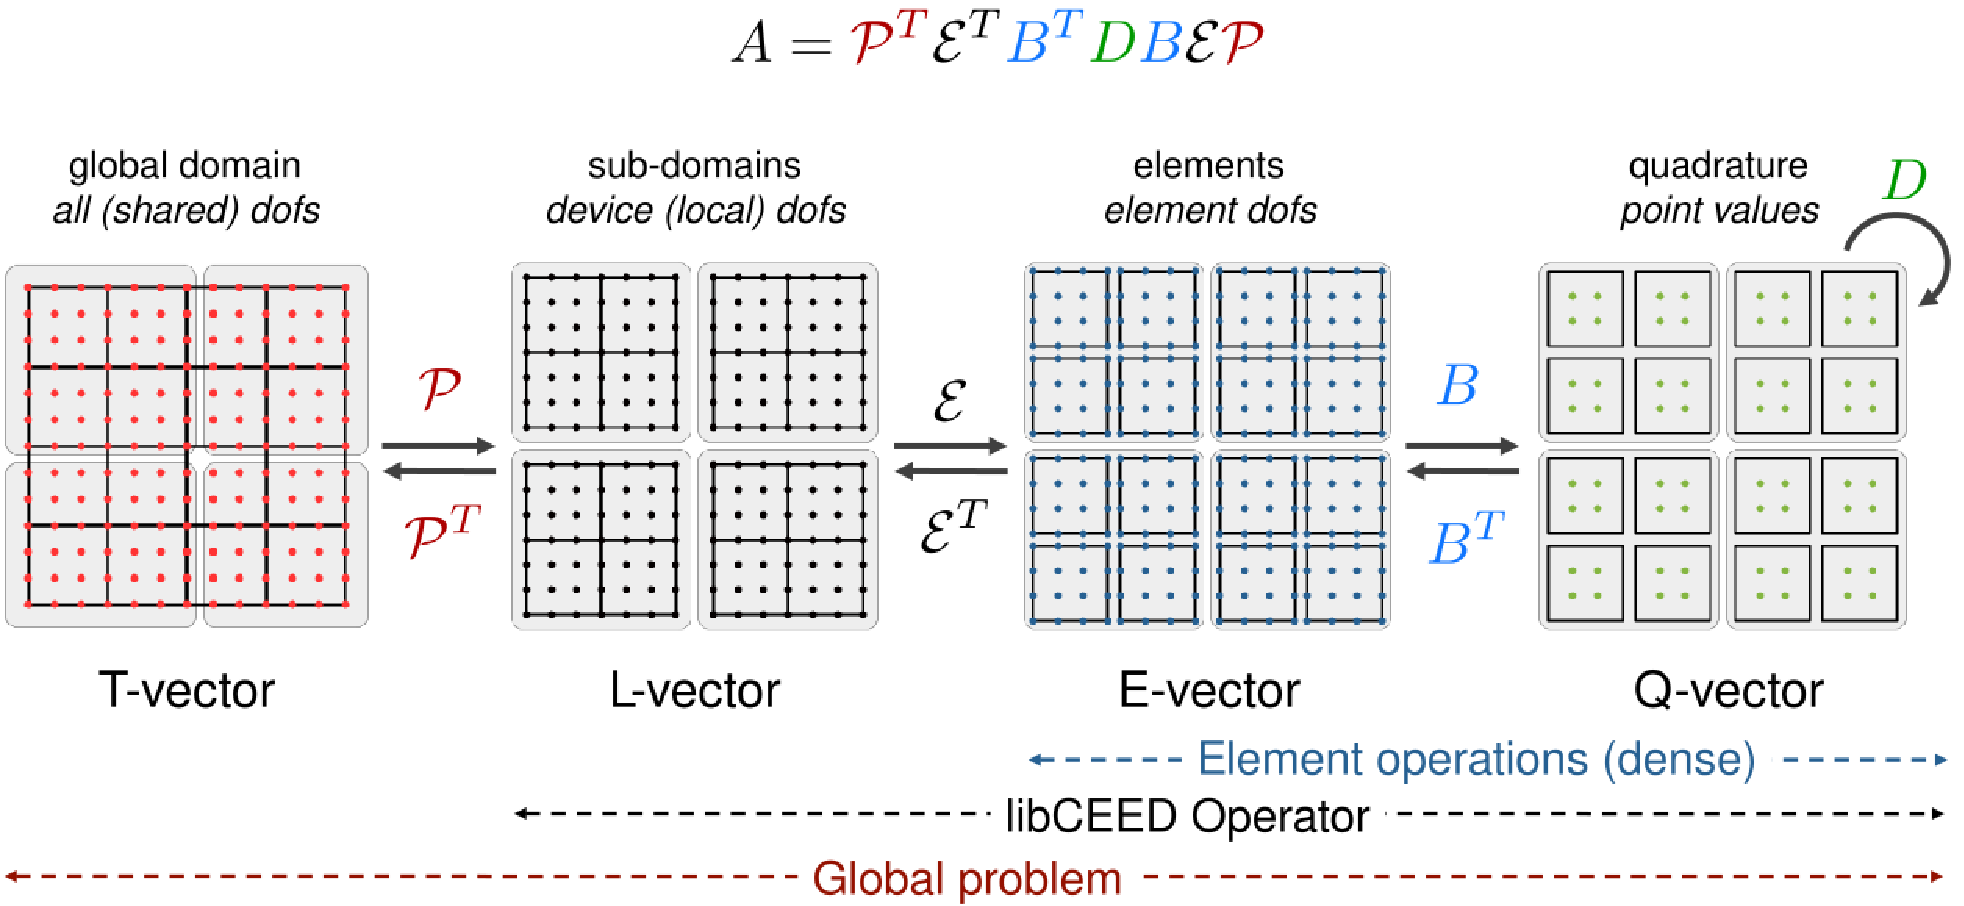
\includegraphics[width=0.9\textwidth]{img/FEMDecomp.pdf}};

    % Create scope with normalized axes
    \begin{scope}[
    x={($0.1*(image.south east)$)},
    y={($0.1*(image.north west)$)}]

    % % Grid
    %     \draw[lightgray,step=1] (image.south west) grid (image.north east);
    %
    % % Axes' labels
    %     \foreach \x in {0,1,...,10} { \node [below] at (\x,0) {\x}; }
    %     \foreach \y in {0,1,...,10} { \node [left] at (0,\y) {\y};}

        \invisible<2->{\draw[ultra thin,white,fill=white] (10, 0.6) rectangle (1.9, 9);}
        \invisible<3->{\draw[ultra thin,white,fill=white] (10, 1.4) rectangle (4.5, 9);}
        \invisible<4->{\draw[ultra thin,white,fill=white] (10, 1.4) rectangle (7.1, 9);}
        \invisible<5->{\draw[ultra thin,white,fill=white] (10, 0) rectangle (0, 2);}
    \end{scope}

    \end{tikzpicture}

\end{frame}

\section{Fluid Simulations with libCEED}

\begin{frame}{Compressible Navier-Stokes}


    \begin{equation*}
        \bm{U}_{,t} + \bm{F}_{i,i}(\bm{U}) - S(\bm{U}) = 0
    \end{equation*}

    for

    \begin{equation*}
        \bm{U} =
        \begin{bmatrix}
            \rho \\
            \rho u_i\\
            E \equiv \rho e
        \end{bmatrix}, \quad
    \bm{F}_i(\bm{U}) =
    \underbrace{
        \begin{pmatrix}
            \rho u_i\\
            \rho u_i u_j + p \delta_{ij} \\
            (\rho e + p)u_i
        \end{pmatrix}}_{\bm F_i^{\text{adv}}} +
    \underbrace{
        \begin{pmatrix}
        0 \\
        -  \sigma_{ij} \\
        - \rho u_i  \sigma_{ij} - k T_{,i}
        \end{pmatrix}}_{\bm F_i^{\text{diff}}}, \quad
    S(\bm{U}) =
    - \begin{pmatrix}
        0\\
        \rho \bm{g} \\
        0
    \end{pmatrix}
    \end{equation*}
\end{frame}

\begin{frame}{Compressible Navier-Stokes for FEM}

    Find \(\bm{U}\in \mathcal{S}^h\)
    \begin{equation*}
        \begin{aligned}
            \int_{\Omega} \bm v \cdot \left( \bm{U}_{,t} - \bm{S}(\bm{U}) \right)  \,\dif \Omega
            - \int_{\Omega} \bm{v}_{,i} \cdot \bm{F}_i(\bm{U})\, \dif\Omega & \\
            + \int_{\partial \Omega} \bm v \cdot \bm{F}_i(\bm{U}) \cdot \widehat{\bm{n}} \,\dif \partial \Omega & \\
            \onslide<2->{\underbrace{+ \int_{\Omega} \mathcal{P}(\bm v)^T \, \left(\bm{U}_{,t} + \bm{F}_{i,i}(\bm{U}) - S(\bm{U})
             \right) \,\dif \Omega}_{\textrm{SUPG}} &= 0 \, , \; \forall \bm v \in \mathcal{V}^h \,}
        \end{aligned}
    \end{equation*}

    \onslide<3->{
        Further simplified into residual form:
        \begin{equation*}
            \mathcal{G}(\bm{U}_{,t}, \bm{U}) = 0
        \end{equation*}
    }
\end{frame}

\begin{frame}{Code Architecture}
    \begin{itemize}
        \item<+-> PETSc used for handling everything libCEED doesn't
            \begin{itemize}
                \item \(\Part, \PartT\) (Partition global-to-local operations)
                \item Time integration, linear, non-linear equation solving
                \item Strong boundary conditions
            \end{itemize}
        \item<+-> PETSc calls a libCEED operator when it needs the residual evaluation
        \item<+-> libCEED Operator based on user-implemented \texttt{CeedQFunction}s (\(\DQfunc\))
            \begin{itemize}
                \item Use different \texttt{CeedQFunction}s for volume vs boundary integrals
                \item Combined into a single \texttt{CeedOperator} to represent \(\mathcal{G}(\bm{U}_{,t}, \bm{U})\)
            \end{itemize}
    \end{itemize}
\end{frame}

\begin{frame}{Time Step Loop}
    \begin{enumerate}
        \item<+-> PETSc gets \(\bm{U}^L = \Part \bm{U}^G\) from current solution
        \item<+-> PETSc calls libCEED to get \(\bm{G}^L = \underbrace{\ElemT \BasT \DQfunc \Bas \Elem}_L \bm{U}^L\)
        \item<+-> PETSc gets \(\bm{G}^G = \PartT \bm{G}^L\)
        \item<+-> PETSc uses \(\bm{G}^G\) to compute new solution value \onslide<+->{...or whatever else it wants}
    \end{enumerate}
\end{frame}

\begin{frame}{Other Misc Things}
    Other features not discussed/shown that are in the libCEED-Fluids example
    \begin{itemize}
        \item Primitive variables
        \item Synthetic turbulence inflow boundary conditions
        \item Shock capturing
    \end{itemize}
\end{frame}

\section*{Questions?}

\end{document}

% \section{A (Very) Brief Finite Element Refresher}
%
% \begin{frame}{Galerkin Form}
%
%         \onslide<+-> {Given the homogenous Poisson equation in weak form: Find \(u \in \mathcal{S}\) such that
%             \begin{equation*}
%                 \int_\Omega v_{,x} u_{,x} \dif \Omega = \int_\Omega vf \dif \Omega \quad \forall v \in \mathcal{V}
%             \end{equation*}}
%
%         \onslide<+-> {
%             Approximate \(\mathcal{S} \approx \mathcal{S}^h = \Span(\{\phi^i\}_i^\ndof)\) and \(\mathcal{V} \approx \mathcal{V}^h = \Span(\{\phi^j\}_j^\ndof)\)
%         }
%         \onslide<+->{
%             \begin{equation*}
%                 \bm{Ax} = \bm{b}
%             \end{equation*}
%         }
%         \onslide<+->{
%             \begin{equation*}
%                 u = \sum_i^\ndof \phi^i x_i \in \mathcal{S}^h, \quad A_{ij} = \int_{\Omega} \phi^i_{,x} \phi^j_{,x} \dif \Omega, \quad b_j = \int_\Omega \phi^j f \dif \Omega
%             \end{equation*}
%         }
%
% \end{frame}
%
% \begin{frame}{Finite Element Method}
%         \onslide<+-> {
%             Discretize the domain \(\Omega\) into elements \(\Omega^e\)
%             \begin{equation*}
%                 \Omega^h = \bigcup_{e=0}^{\nelm} \Omega^e \approx \Omega
%             \end{equation*}
%         }
%         % \onslide<+-> {
%         %     Define finite element function spaces:
%         %     \begin{equation*}
%         %         \mathcal{S}^h \coloneqq \left\{ v^h \in \mathcal{F}(\Omega^h)\right\}
%         %     \end{equation*}
%         % }
%         % \onslide<+-> {
%         %     \begin{equation*}
%         %         A_{ij} = \sum_e^\nelm \int_{\Omega^e} \phi^i_{,x} \phi^j_{,x} \dif \Omega, \quad b_j = \sum_e^\nelm \int_{\Omega^e} \phi^j f \dif \Omega
%         %     \end{equation*}
%         % }
%         \onslide<+->{
%             Approximate the integrals over elements via quadrature \[\int g(x) \dif x \approx \sum_k^\nquad w^k g(\xi^k)\]
%         }
%         \onslide<+->{
%             Thus the final problem can be stated as: Find \(\bm{x} \in \mathbb{R}^\ndof\) in \(\bm{Ax} = \bm{b}\) for
%             \begin{equation*}
%                 A_{ij} = \sum_e^\nelm \sum_k^\nquad \left[ w^k \phi^i_{,x}(\xi^k) \phi^j_{,x}(\xi^k) \right]_{\Omega^e}, \quad b_j = \sum_e^\nelm \sum_k^\nquad \left[ w^k \phi^j(\xi^k) f(\xi^k) \right]_{\Omega^e}
%             \end{equation*}
%         }
%
% \end{frame}


% ------------ Backup slides (old ones that may get reused later)
% \begin{frame}{libCEED Operator}
%
%     \begin{columns}
%         \column{0.4\textwidth}
%         \begin{center}
%             \begin{tabular}{ c c c }
%             Operator & libCEED Object\\ [0.5ex]
%             \hline\hline
%             \onslide<+->{\(\Elem\)   & \footnotesize\texttt{CeedElemRestriction} \\}
%             \onslide<+->{\(\Bas\)    & \footnotesize\texttt{CeedBasis} \\}
%             \onslide<+->{\(\DQfunc\) & \footnotesize\texttt{CeedQFunction} \\}
%             \onslide<+->{\(\ElemT\BasT\DQfunc\Bas\Elem\) & \footnotesize\texttt{CeedOperator}}
%             \end{tabular}
%         \end{center}
%
%         \column{0.6\textwidth}
%             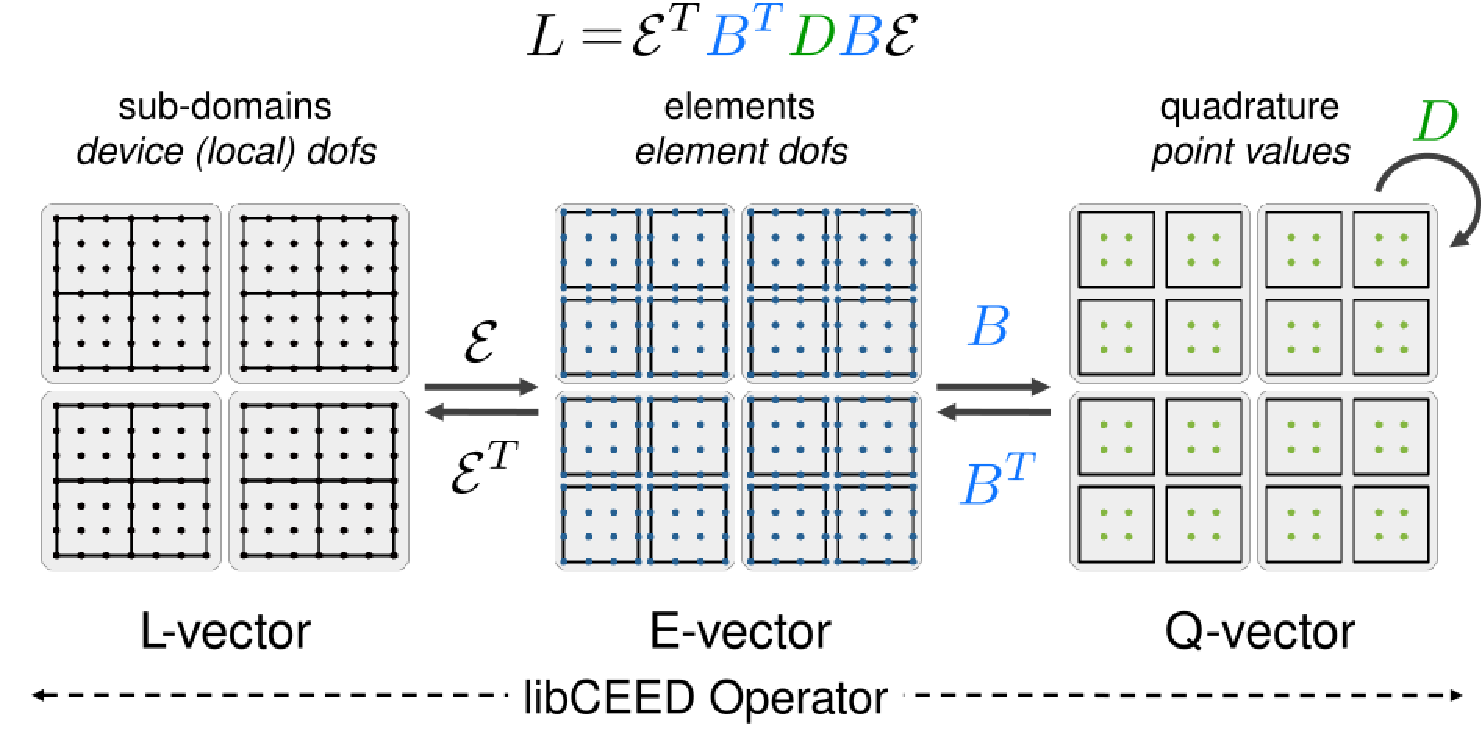
\includegraphics[width=\textwidth]{img/libCEED_Operator.pdf}
%     \end{columns}
%     \begin{block}{Note}<+->
%         libCEED implements the operators matrix-free; None of the libCEED Objects store a matrix
%     \end{block}
% \end{frame}

% \begin{frame}{Defining the libCEED Operator}
%
%     \begin{columns}
%         \column{0.5\textwidth}
%         \onslide<1->{
%             \footnotesize\texttt{CeedElemRestriction}
%             \begin{itemize}
%                 \item Defined by element connectivity and the number of components
%             \end{itemize}
%         }
%         \onslide<2->{
%             \footnotesize\texttt{CeedBasis}
%             \begin{itemize}
%                 \item Defined by the basis functions and the quadrature rule
%                 \item Built-in options for common basis functions and quadrature rules
%             \end{itemize}
%         }
%
%         \column{0.5\textwidth}
%         \onslide<3->{
%             \footnotesize\texttt{CeedQFunction}
%             \begin{itemize}
%                 \item C function
%                 \item Common operators available (mass, poisson, identity, etc.)
%                 \item User defined QFunctions also possible
%             \end{itemize}
%         }
%
%         \onslide<4->{
%             \footnotesize\texttt{CeedOperator}
%             \begin{itemize}
%                 \item Computation backend defined at runtime
%                 \item Full \(L\) operator (can be) JITed to the desired backend (CUDA, HIP, CPU, etc.)
%             \end{itemize}
%         }
%     \end{columns}
% \end{frame}

% \begin{frame}[fragile]{Poisson CeedQFunction}
%     \begin{columns}
%
%         \column{0.4\textwidth}
%         \onslide<1->{
%             \[ \sum_k^\nquad \left[ w^k u_{,x}(\xi^k) v_{,x}(\xi^k) \right]_{\Omega^e} \]
%             \vspace{-20pt}
%             \[\BasT\DQfunc\Bas\]
%         }
%         \vspace{-20pt}
%         \begin{itemize}
%             \item<2-> \texttt{ug=} \(u_{,x}(\xi^k) = \Bas u^e\)
%             \item<3-> \texttt{q\char`_data=} \(w^k\)\footnote<3->{along with jacobian determinant}
%             \item<4-> \texttt{vg=} \(w^k u_{,x}(\xi^k) = \DQfunc\Bas u^e\)
%             \item<5-> \(w^k u_{,x}(\xi^k) v_{,x}(\xi^k) = \BasT \DQfunc \Bas u^e\)
%         \end{itemize}
%
%     \column{0.6\textwidth}
% % \onslide<2->{
% \begin{ccode}
% CEED_QFUNCTION(Poisson1DApply)(void *ctx, const CeedInt Q,
%                                const CeedScalar *const *in,
%                                CeedScalar *const *out) {
%   // in[0] is gradient u, size (Q)
%   // in[1] is quadrature data, size (Q)
%   const CeedScalar *ug = in[0], *q_data = in[1];
%
%   // out[0] is output to multiply against gradient v, size (Q)
%   CeedScalar *vg = out[0];
%
%   // Quadrature point loop
%   CeedPragmaSIMD
%   for (CeedInt i=0; i<Q; i++) {
%     vg[i] = ug[i] * q_data[i];
%   } // End of Quadrature Point Loop
%
%   return CEED_ERROR_SUCCESS;
% }
% \end{ccode}
% % }
%
%     \end{columns}
% \end{frame}
